\documentclass[tikz,border=8pt]{standalone}
\usepackage{xcolor}
\usetikzlibrary{arrows.meta, shapes.geometric}

\definecolor{iiitblue}{RGB}{10,55,120}
\definecolor{controllercolor}{RGB}{95,40,140}
\definecolor{actioncolor}{RGB}{10,120,100}

\begin{document}
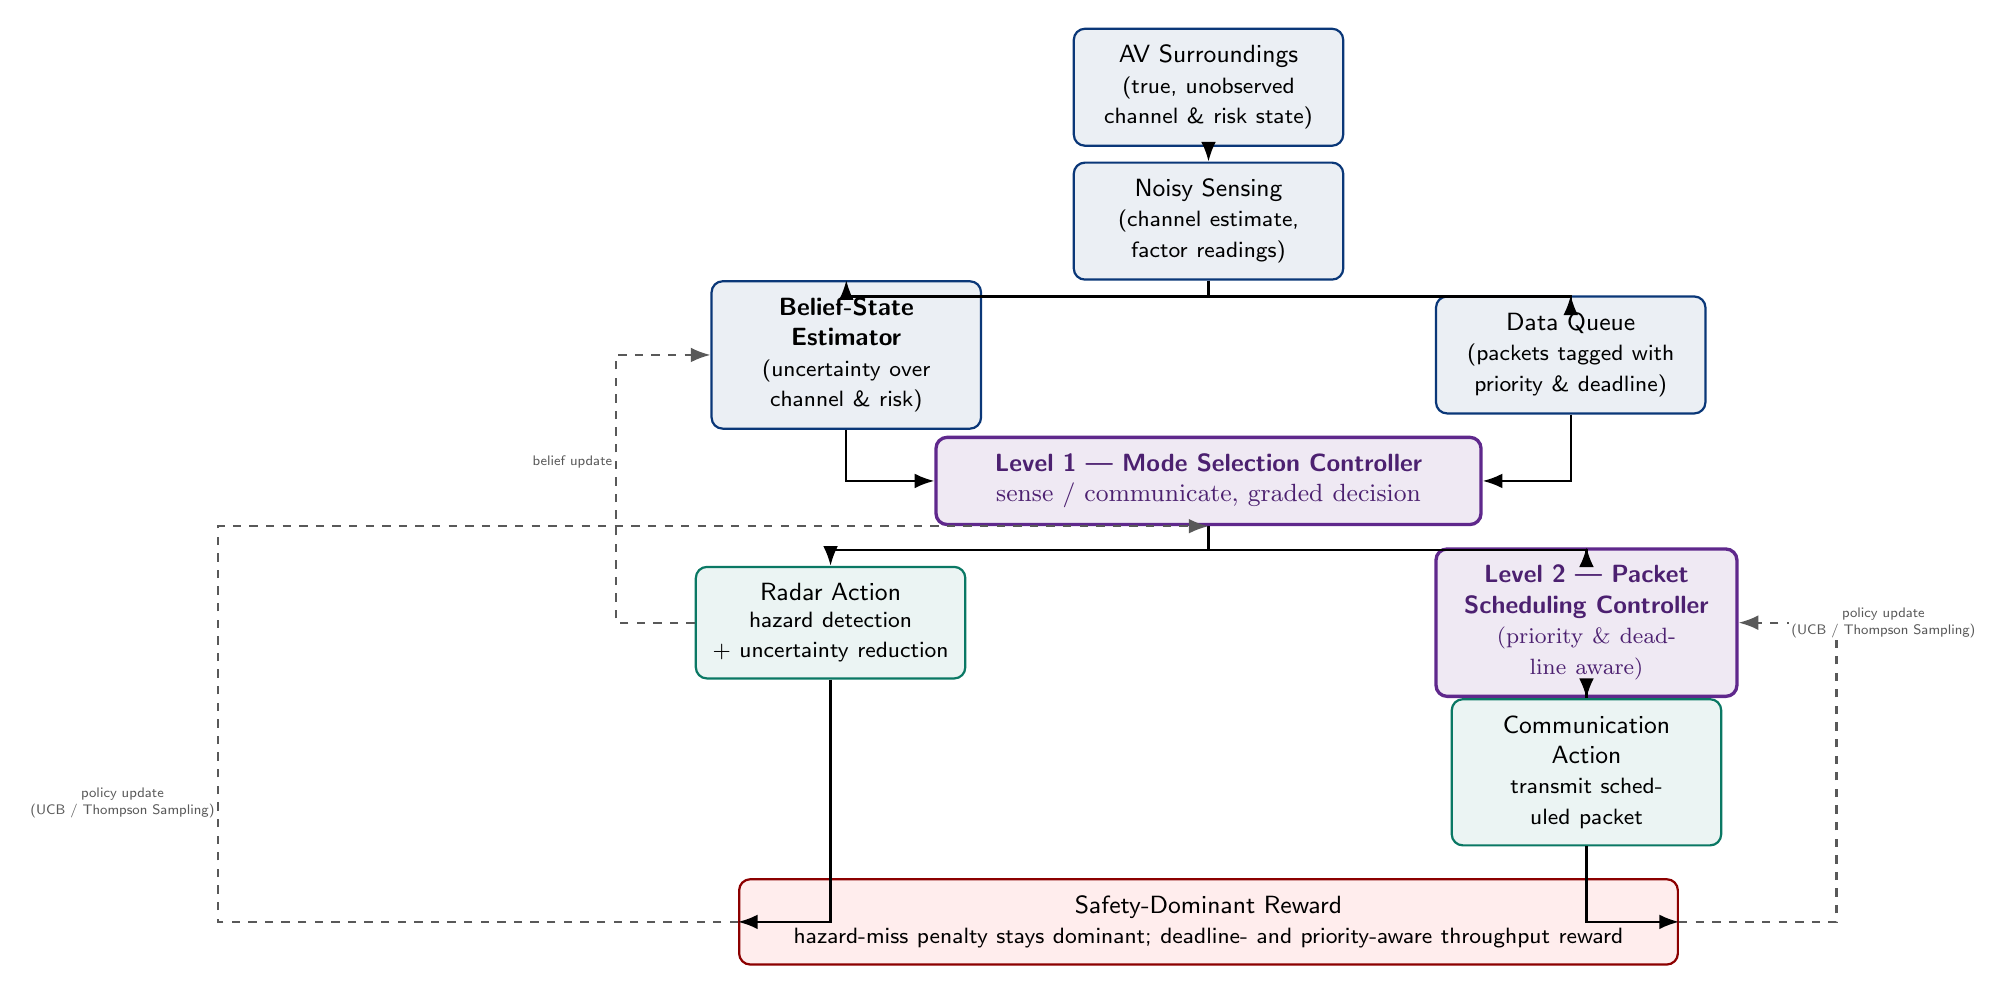
\begin{tikzpicture}[
  font=\sffamily,
  inner sep=6pt,
  box/.style={draw=iiitblue, thick, rounded corners, fill=iiitblue!8,
    align=center, minimum height=0.9cm, text width=3.0cm, font=\sffamily\small},
  controller/.style={draw=controllercolor, very thick, rounded corners, fill=controllercolor!10,
    align=center, minimum height=0.9cm, text width=3.4cm, font=\sffamily\small\bfseries, text=controllercolor!80!black},
  actionbox/.style={draw=actioncolor, thick, rounded corners, fill=actioncolor!8,
    align=center, minimum height=0.9cm, text width=3.0cm, font=\sffamily\small},
  rewardbox/.style={draw=red!55!black, thick, rounded corners, fill=red!7,
    align=center, minimum height=0.9cm, text width=11.5cm, font=\sffamily\small},
  arr/.style={-{Latex[length=2.5mm]}, thick},
  fb/.style={-{Latex[length=2.5mm]}, thick, dashed, gray!70!black},
]

% --- Top: environment and sensing ---
\node[box] (env) at (0,0) {AV Surroundings\\\footnotesize (true, unobserved channel \& risk state)};
\node[box] (sense) at (0,-1.7) {Noisy Sensing\\\footnotesize (channel estimate, factor readings)};

% --- Belief state + queue ---
\node[box] (belief) at (-4.6,-3.4) {\textbf{Belief-State Estimator}\\\footnotesize (uncertainty over channel \& risk)};
\node[box] (queue) at (4.6,-3.4) {Data Queue\\\footnotesize (packets tagged with priority \& deadline)};

% --- Level 1 controller ---
\node[controller, text width=6.5cm] (l1) at (0,-5.0) {Level 1 --- Mode Selection Controller\\\normalfont sense / communicate, graded decision};

% --- Branches ---
\node[actionbox] (radar) at (-4.8,-6.8) {Radar Action\\\footnotesize hazard detection\\\footnotesize $+$ uncertainty reduction};
\node[controller] (l2) at (4.8,-6.8) {Level 2 --- Packet\\Scheduling Controller\\\normalfont\footnotesize (priority \& deadline aware)};
\node[actionbox] (comm) at (4.8,-8.7) {Communication Action\\\footnotesize transmit scheduled packet};

% --- Reward ---
\node[rewardbox] (reward) at (0,-10.6) {Safety-Dominant Reward\\\footnotesize hazard-miss penalty stays dominant; deadline- and priority-aware throughput reward};

% --- Forward arrows ---
\draw[arr] (env) -- (sense);
\draw[arr] (sense.south) -- ++(0,-0.2) -| (belief.north);
\draw[arr] (sense.south) -- ++(0,-0.2) -| (queue.north);
\draw[arr] (belief.south) |- (l1.west);
\draw[arr] (queue.south) |- (l1.east);
\draw[arr] (l1.south) -- ++(0,-0.3) -| (radar.north);
\draw[arr] (l1.south) -- ++(0,-0.3) -| (l2.north);
\draw[arr] (l2) -- (comm);
\draw[arr] (radar.south) |- (reward.west);
\draw[arr] (comm.south) |- (reward.east);

% --- Feedback arrows ---
\draw[fb] (radar.west) -- ++(-1.0,0) |- node[pos=0.3, left, font=\sffamily\tiny, fill=white, inner sep=1pt] {belief update} (belief.west);
\draw[fb] (reward.west) -- ++(-6.6,0) |- node[pos=0.15, left, font=\sffamily\tiny, fill=white, inner sep=1pt, align=center] {policy update\\(UCB / Thompson Sampling)} (l1.south);
\draw[fb] (reward.east) -- ++(2.0,0) |- node[pos=0.75, right, font=\sffamily\tiny, fill=white, inner sep=1pt, align=center] {policy update\\(UCB / Thompson Sampling)} (l2.east);

\end{tikzpicture}
\end{document}
